\documentclass[xelatex,11pt, xcolor=dvipsnames]{beamer}
\usepackage{pgfpages}
\usepackage{fontspec}
\usepackage{polyglossia}
\PolyglossiaSetup{french}{indentfirst=false}
\usepackage[french=guillemets]{csquotes}
\usepackage{xpatch}
\usepackage{diagbox}

\setmainlanguage{french}
\xapptocmd\ttfamily{\XeTeXinterchartokenstate=0 }{}{}
\newcommand{\nospace}[1]{\texttt{#1}}

\usepackage{algorithm}
\usepackage[noend]{algpseudocode}
    \newcounter{lastenum}
    \newcommand{\mtpause}{\setcounter{lastenum}{\value{enumi}}}
    \newcommand{\mtresume}{\setcounter{enumi}{\value{lastenum}}}
\resetcounteronoverlays{lastenum}

\usepackage[backend=biber]{biblatex}
\addbibresource{Modele.bib} 
\bibliography{Modele}
\setbeamertemplate{bibliography item}[triangle]

\usepackage{multirow} % row fusion
\usepackage{array} % column fusion
\usepackage{xfrac} % small fractions
\usepackage{adjustbox}
\usepackage{listings}
\usepackage{dirtree}

\usetheme{Warsaw}
\usecolortheme{wolverine}

\setbeamertemplate{frametitle}{
	\nointerlineskip  
	\begin{beamercolorbox}[wd=\paperwidth,ht=2.75ex,dp=1.375ex]{frametitle}
		\hspace*{2ex}\insertframetitle \hfill {
			\small\insertframenumber/\inserttotalframenumber
		} \hspace*{1ex}%
    	\end{beamercolorbox}
}

 \titlegraphic{\vspace{-1cm}
      
\includegraphics[width=2.5cm]{images/paris8_1}\hspace*{4.75cm}~%
      \hfill
      
\includegraphics[width=2.5cm]{images/logo}
}

\beamertemplatenavigationsymbolsempty
\setbeamertemplate{blocks}[rounded][shadow=true]
\setbeamerfont{page number in head/foot}{size=\large}

% Parties conditionnelles
\usepackage{etoolbox} % pour toggle
\newtoggle{bandeaularge}
\newtoggle{MSsanspuces}


% Ici on choisit si on veut un bandeau en largeur (pas de sous section) ou normal
\toggletrue{bandeaularge}% commenter pour passer au bandeau normal

% Bandeau en largeur
\iftoggle{bandeaularge}
{%
  \setbeamertemplate{headline}{%
    \hbox{%
      \begin{beamercolorbox}[wd=\paperwidth, ht=2.8ex, dp=1ex]{section in head/foot}%
      \insertsectionnavigationhorizontal{\paperwidth}{}{}%
      \end{beamercolorbox}%
  }%
}%
\setbeamertemplate{section in head/foot}%
{\colorbox{yellow!90!orange}{\insertsectionhead}}%
% Essai pour élargir le titre courant mais pas terrible
%\setbeamertemplate{section in head/foot}{\colorbox{yellow!90!orange}{\parbox{10em}{\centering\color{black}\insertsectionhead\par}}}
}%{}

\iftoggle{MSsanspuces}{%
\setbeamertemplate{itemize items}[bullet]}{}

\subtitle{Cours Ingénierie des langues\\\textbf{Projet, 1ère phase}}
\institute{\normalsize Université Paris 8, LIASD\\
Licence d'informatique}

% Les utilisateurs sous Windows qui ne voient pas de puces doivent décommenter la ligne suivante
%\toggletrue{MSsanspuces}

% Ici on choisit si on veut seulement les diapos ou le texte à lire sur son écran

\setbeameroption{hide notes} % Only slides
%\setbeameroption{show only notes} % Only notes
%\setbeameroption{show notes on second screen=right} % Both

% Ici on indique son titre et son nom

\title{Extraire les données de mails pour déterminer si c'est un spam}
\author[\textsc{M. Goehry}]{\textsc{Martial Goehry}}


\begin{document}
{ \setbeamertemplate{headline}{}
  \setbeamertemplate{footline}{}
  \begin{frame}
  \titlepage
  \end{frame}

\note{
}
}

\begin{frame}{Plan}
  \tableofcontents[sectionstyle=show/show, hidesubsections]
\note{
}  
\end{frame}

\section{Objectif}

\begin{frame}{Objectif}
  \begin{block}{}
  L'objectif est d'extraire des données d'e-mails pour déterminer s'ils sont des spams.
  \end{block}
  \begin{itemize}
  \item langue concernée : Anglais
  \item type de corpus : corpus monolingue écrit
  \item type de données : e-mail
  \end{itemize}
\end{frame}

\section{Corpus}

\begin{frame}{Corpus}
	\begin{block}{Dataset de mail du projet SpamAssassin}
		\begin{itemize}
			\item Anglais
			\item \url{https://spamassassin.apache.org/old/publiccorpus/}
			\item consulté le 27/01/2022
			\item 6065 fichiers email déjà trier en ham et spam
		\end{itemize}
	\end{block}
	
	\begin{block}{Dataset de mail de la compagnie Enron}
		\begin{itemize}
			\item Anglais
			\item \url{https://www.kaggle.com/wcukierski/enron-email-dataset}
			\item consulté le 27/01/2022
			\item fichier CSV avec 33 834 245 lignes (un mail par ligne) non trier
		\end{itemize}
	\end{block}
\end{frame}

\section{Difficultés}

\begin{frame}{Analyse des sites}
  Je n'ai pas réussi à trouver de dataset de mail en français, j'ai donc du me retourner vers les dataset en anglais.
\end{frame}

\section{Aspiration}

\begin{frame}{Aspiration}
	J'ai recherché un outil simple me permettant d'extraire facilement le message d'un mail en faisant abstraction du nombre important de métadonnées associées. Mon choix s'est porté sur le module \emph{email} de python. Je me suis donc orienté vers une solution tout python pour le traitement des données. \\
	Déroulé :
	\begin{enumerate}
		\item Chargement des données brutes à l'aide de python.
		\item Utilisation du module \emph{email} pour importer et transformer les fichiers textes et csv en objet \emph{email.message}.  
	\end{enumerate}
\end{frame}

\begin{frame}{Aspiration}
	\begin{block}{Fichiers textes, SpamAssassin}
	Chaque mail est stocké dans un fichier texte. Ces fichiers sont déjà triés en spam et non spam (ham).
	Une fois le fichier ouvert j'utilise la fonction \emph{email.message\_from\_string()}
	\end{block}
	
	\begin{block}{Fichier CSV, compagnie Enron}
	Importation du fichier CSV avec le module \emph{csv} de python.
	Seulement 2 colonnes sont présentes : chemin, message.\\
	Pour chaque ligne on applique la fonction \emph{email.message\_from\_string()} à la partie correspondante au message.
	\end{block}
	
	A partir de ce point je ne traite plus que des objets \emph{email.message}
	
\end{frame}

\begin{frame}{Aspiration, difficultés} 
	\begin{block}{Encodage}
	Certains encodages ne sont pas pris en charge par le module \emph{email}. J'ai du me limiter aux encodages suivants : ascii, Windows-1252, ISO-8859-1, utf-8.\\
	J'utilise le module \emph{chardet} pour faire la détection de l'encodage
	\end{block}
	
	\begin{block}{Multiple charset}
	Les messages mails peuvent avoir plusieurs charset à l'intérieur du payload (\emph{get\_content\_charset}). Les charset suivant m'ont posé des problèmes lors du traitement, j'ai du les écarter : unknown-8bit, default, default\_charset, gb2312\_charset, chinesebig5, big5.\\
	Écarter ces charset me permet d'enlever les messages écrits en turc, chinois ou japonais. 
	\end{block}
	
\end{frame}

\begin{frame}{Extraction des données}
	Une fois le message disponible, le module email se charge de convertir la chaîne de caractère en objet \emph{email.Message}. De cet objet on va pouvoir extraire les données suivantes:
	\begin{itemize}
		\item objet du mail (Subject)
		\item expéditeur (From)
		\item corps du mail (payload)
	\end{itemize}
	Il est possible que le corps du mail soit séparé en plusieurs sous-partie (multi-part).
	Dans ce cas il faut concaténer les parties textuelles. 
	\begin{itemize}
		\item text/plain
		\item text/html
		\item text/enriched
	\end{itemize}
	Les types html et enriched ont un pré-nettoyage pour retirer les balises. 
\end{frame}

\section{Nettoyage}

\begin{frame}{Nettoyage}
  Les messages étant déjà chargés dans le programme en python j'ai trouvé préférable d'effectuer toutes les opérations de nettoyage directement après la phase d'importation. \\
  
	Étapes du nettoyage du texte:
	\begin{enumerate}
		\item Suppression des balises html avec le module \emph{BeautifulSoup} (bs4)
		\item Suppression des balises eniched text avec le module \emph{re}
		\item Tout le texte en minuscule avec la méthode lower()
		\item Suppression des réponses avec le module \emph{re}
		\item Substitutions des adresses mail, url et numéro de téléphone avec le module \emph{re}
		\item Substitutions des prix et des nombres avec le module \emph{re}
		\item Suppression des ponctuations superflues avec le module \emph{re}
	\end{enumerate}

\end{frame}
	
\begin{frame}[fragile]{Expressions régulières}
	\begin{itemize}
		\item Capture des balises enriched text: \verb'<.*>'
		\item Capture des réponses: \verb'^>.*$'
		\item Capture mail: \verb'[a-zA-Z0-9_.+-]+@[a-zA-Z0-9-]+\\.[a-zA-Z0-9-.]+'
		\item Capture url: \verb'(http|ftp|https)?:\/\/([\w\-_]+(?:(?:\.[\w\-_]+)+))'
							\verb'([\w\-\.,@?^=%&:/~\+#]*[\w\-\@?^=%&/~\+#])?'
		\item Capture téléphone1: \verb'\\(\\d{3}\\)\\d+-\\d+'
		\item Capture téléphone2: \verb'\\+\\d+([ .-]?\\d)+'
		\item Capture prix1: \verb'[$€£]( )?\\d+([.,]\\d+)? '
		\item Capture prix2: \verb' \\d+([.,]\\d+)?( )?[$€£]'
		\item Capture nombre: \verb'\\d+'
	\end{itemize}
\end{frame}

\begin{frame}{Exemple de nettoyage texte brut}
	\begin{block}{Brut}
Message dedicated to be a sample to show how the process is clearing the text.

Begin reply :
> He once said
>>> that it would be great
End of reply.
Substitutions :
spamassassin-talk@example.sourceforge.net
https://www.inphonic.com/r.asp?r=sourceforge1\&refcode1=vs33
hello.foo.bar
between \$ 25 and 25,21 \$

A number is : 2588,8 588
Phone type a : (359)1234-1000
Phone type b : +34 936 00 23 23
Ponctuation : ----\#\# ..
	\end{block}
		
	\begin{block}{Nettoyé}
message dedicated to be a sample to show how the process is clearing the text. begin reply end of reply. substitutions MAIL URL URL between PRIX and PRIX a number is NOMBRE , NOMBRE NOMBRE phone type a TEL phone type b TEL ponctuation . 
	\end{block}

\end{frame}

\begin{frame}{Nettoyage enriched text}

	\begin{block}{Brut}
	<smaller>I'd like to swap with someone also using Simple DNS to take
advantage of the trusted zone file transfer option.</smaller>
	\end{block}
	
	\begin{block}{Nettoyé}
	I'd like to swap with someone also using Simple DNS to take
advantage of the trusted zone file transfer option.
	\end{block}
	
\end{frame}

\begin{frame}[fragile]{Nettoyage HTML brut}
\small
\begin{verbatim}
<!DOCTYPE html PUBLIC "-//W3C//DTD HTML 4.01 Transitional//EN">
<html>
<head>
  <title>Foobar</title>
</head>
<body>
I actually thought of this kind of active chat at AOL 
bringing up ads based on what was being discussed and 
other features
  <pre wrap="">On 10/2/02 12:00 PM, "Mr. FoRK" 
  <a class="moz-txt-link-rfc2396E"href="mailto:fork_
  list@hotmail.com">&lt;fork_list@hotmail.com&gt;</a> 
  wrote: Hello There, General Kenobi !?
<br>
</body>
</html>
\end{verbatim}
\normalsize
	
\end{frame}

\begin{frame}[fragile]{Nettoyage HTML nettoyé}
\small
\begin{verbatim}
Foobar


I actually thought of this kind of active chat at AOL 
bringing up ads based on what was being discussed and 
other features
  On 10/2/02 12:00 PM, "Mr. FoRK" 
   
  wrote: Hello There, General Kenobi !?
\end{verbatim}
\normalsize
\end{frame}

\begin{frame}{Conclusion nettoyage}
	Le nettoyage du texte s'arrête avant l'étape de lemmatisation. 
	Initialement, je souhaitais réaliser cette étape avant le stockage, 
	mais j'ai peur qu'une réduction trop importante n'altère le résultat de recherche de sentiment.\\
	
	Je garde donc le texte avec une structure permettant d'en comprendre le sens. \\
	
	Point à améliorer :
	\begin{itemize}
		\item Les mails que j'ai pu collecter contiennent des exemples de code en C que je n'ai pas été en mesure de retirer.
		\item Récupérer les redirections mail et URL dans les balises HTML
 	\end{itemize}  
\end{frame}


\section{Stockage}

\begin{frame}{Moteur de base de données}
  \begin{itemize}
  \item Base de données choisie : ElasticSearch
  \item Raisons de ce choix : J'avais envie de travailler avec une base de données NoSQL.
  		L'utilisation du format JSON est assez souple et s'intègre bien avec python. 
  		L'interface graphique, Kibana, permet déjà une prévisualisation des données. 
  		ElasticSearch intègre nativement un moteur Lucene pour l'indexation des données textuelles. 
  		Il devrait être possible d'utiliser ce moteur pour faire l'analyse de sentiment, ou d'extraire les message pour les traiter avec un autre outil de traitement du langage.
  \item Résultat : J'ai pu récupérer et stocker le corps de 254 740 mails ainsi que quelques informations statistiques (nombre de mots, nombre de substitutions) et des informations de ciblage (adresses mail, sujet). L'indice de cette base occupe un espace de 448.53 Mb.
  \end{itemize}
\end{frame}

\begin{frame}
	Avant d'utiliser sur le moteur ElasticSearch, j'avais choisis une base PostgreSQL avec une opération de tokenisation au préalable. J'ai abandonnée cette solution car:
	\begin{itemize}
		\item Temps de chargement des données dans la base : 2 jours contre 1 heure avec Elastic
		\item Taille de la base : 1.6G contre 448M avec Elastic
		\item Difficulté de reconstitution du message original
	\end{itemize}
	Il était cependant plus facile d'obtenir les statistiques suivantes :
	\begin{itemize}
		\item Nombre de mots uniques dans le corpus et dans chaque document
		\item Nombre de d'occurrences d'un mot dans le corpus ou dans chaque document
	\end{itemize}
\end{frame}


\begin{frame}
	Données à stockées au format JSON dans une base ElasticSearch avec le mappage :
	\dirtree{%
		.1 document.
		.2 hash : empreinte en md5.
		.2 chemin : accès au fichier brut.
		.2 categorie : ham, spam ou inconnu.
		.2 sujet : objet du mail.
		.2 expediteur : champ FROM.
		.2 nombres\_mots : nombre de mots dans le corps.
		.2 substitutions : remplacement dans le corps.
		.3 URL : liens URL.
		.3 MAIL : adresses mails.
		.3 TEL : numéros de téléphone.
		.3 NOMBRE : chiffres sans indication monétaire.
		.3 PRIX : chiffres avec des indications monétaire.
		.2 message : corps du mail.
	}
	
\end{frame}


\section{Caractéristiques}

\begin{frame}{Caractéristiques}
	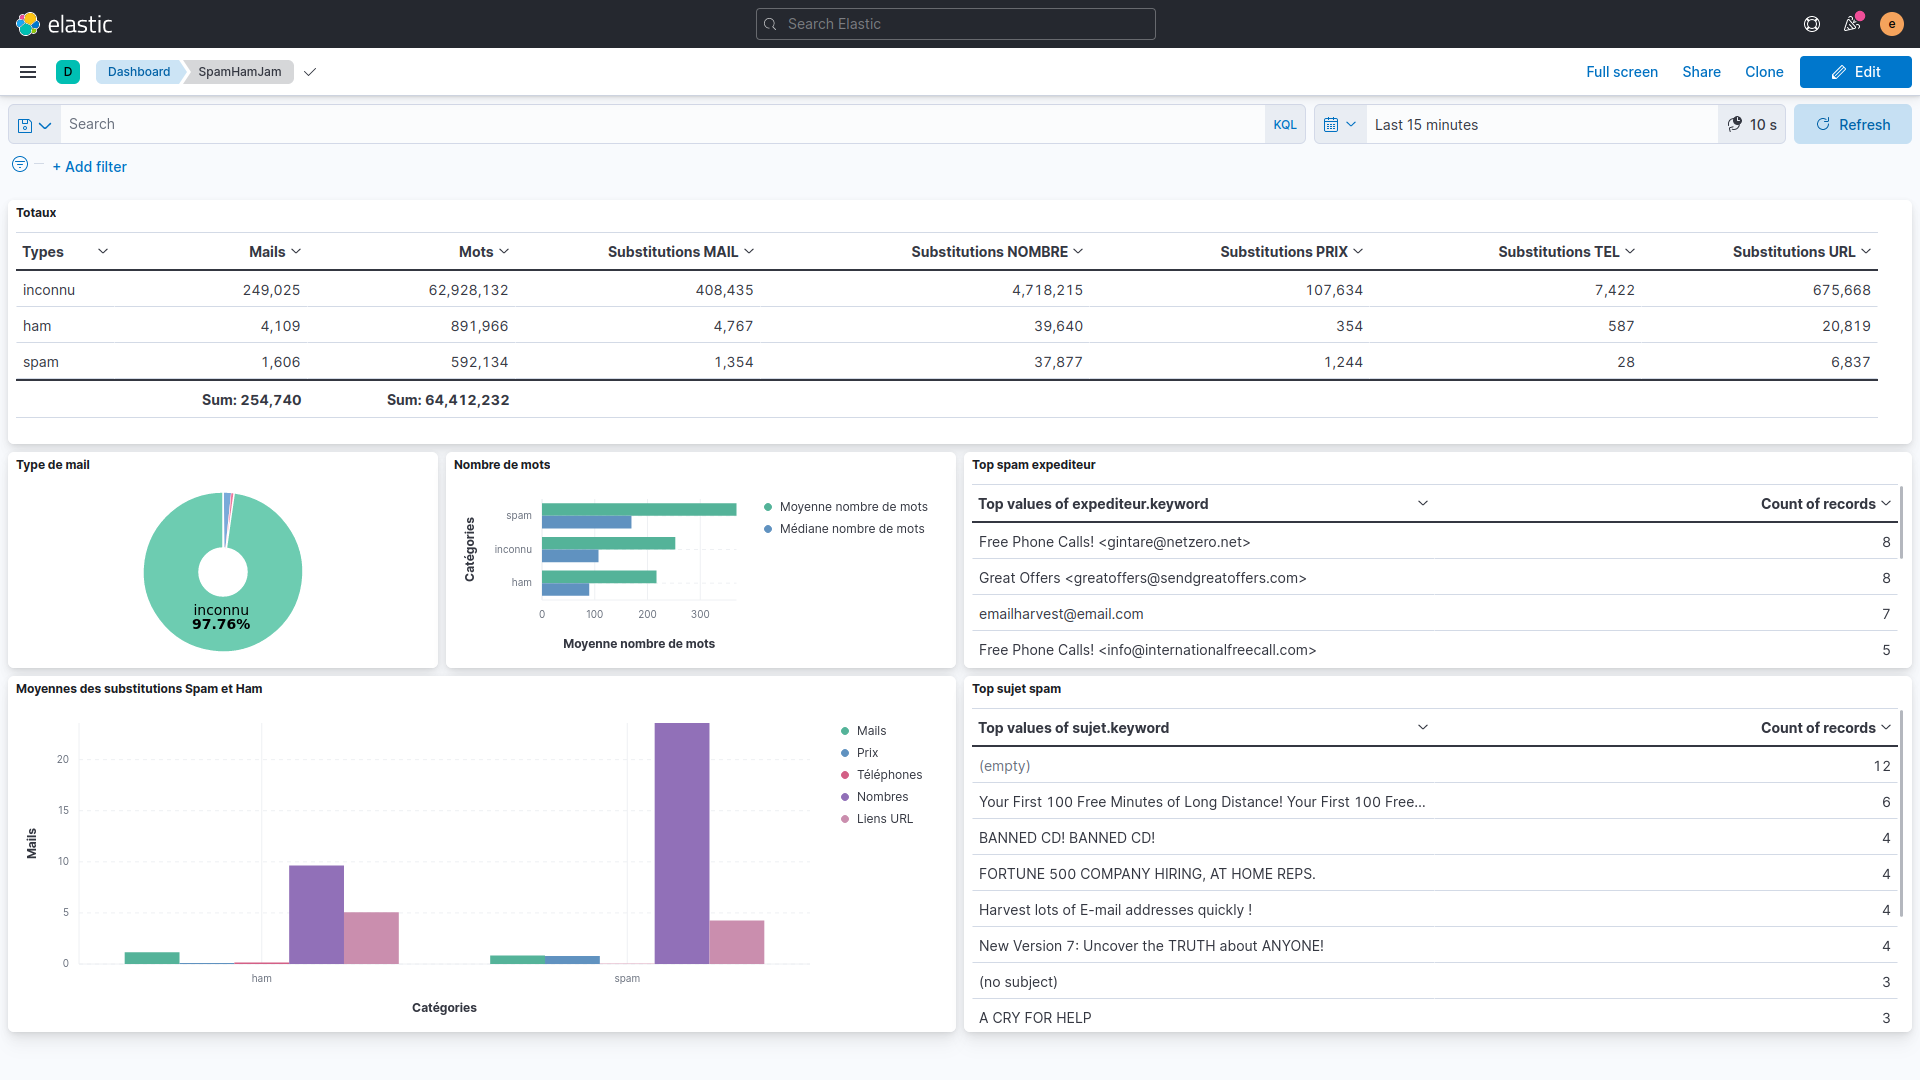
\includegraphics[width=\linewidth]{images/dashboard.png}
\end{frame}


\section{Conclusion}
  \begin{frame}
  \begin{block}{Conclusion}
  %Ici une conclusion qui met en valeur votre travail et annonce les questions que vous vous posez et ce que vous prévoyez de faire.
  Je pense avoir réussi à faire une chaîne d'opérations sur mails (récupération, nettoyage, stockage) qui devrait me permettre de maintenir un traitement uniforme dans la durée.\\
  
  Je me suis directement orienté vers une solution complète en python, même si la majeure partie de mes traitement aurait pu être fait avec \emph{sed} ou \emph{awk}.
  \end{block}
  \begin{block}{La suite}
  La prochaine étape va être de pouvoir faire l'analyse de sentiment à proprement parler.
  Le scoring que j'espère récupérer devrait pouvoir me permettre d’entraîner un modèle pour pouvoir affiner la détection des spams.
  \end{block}
  \end{frame}

% éléments hors section
\appendix

  \begin{frame}{Références}%[allowframebreaks]
  \renewcommand*{\bibfont}{\footnotesize}
  \nocite{*}
  \printbibliography[heading=none]
  \begin{itemize}
  	\item Documentation du paquet email de python, [en ligne], \url{https://docs.python.org/fr/3/library/email.html} (27/01/2022)
  	\item Documentation du paquet regex de python, [en ligne], \url{https://docs.python.org/fr/3/library/re.html} (30/01/2022)
  	\item Documentation du paquet beautifulsoup, extraire du texte de l'html, [en ligne], \url{https://beautiful-soup-4.readthedocs.io/en/latest/} (30/01/2022)
  	\item Expression régulière URL, [en ligne], capturer les URL \url{https://www.i2tutorials.com/match-urls-using-regular-expressions-in-python/} (30/01/2022)
  \end{itemize}
\end{frame}

  \begin{frame}{Références}%[allowframebreaks]
  \renewcommand*{\bibfont}{\footnotesize}
  \nocite{*}
  \printbibliography[heading=none]
  \begin{itemize}
  	\item Détecter l'encodage d'un texte, [en ligne], \url{https://chardet.readthedocs.io/en/latest/usage.html} (03/02/2022)
  	\item Installer ElasticSearch avec docker, [en ligne], \url{https://www.elastic.co/guide/en/elasticsearch/reference/current/docker.html} (01/04/2022)
  	\item Documentation python module ElasticSearch, [en ligne], \url{https://elasticsearch-py.readthedocs.io/en/v8.1.3/} (01/04/2022)
  	\item Nettoyage de texte en python, [en ligne], \url{https://www.machinelearningplus.com/nlp/lemmatization-examples-python/}       (28/01/2022)
  \end{itemize}
\end{frame}

\begin{frame}
  \begin{block}{}
  \centering
  Merci pour votre attention
  \end{block}
\end{frame}


\end{document}
